\documentclass[
10pt, % Main document font size
a4paper, % Paper type, use 'letterpaper' for US Letter paper
oneside, % One page layout (no page indentation)
%twoside, % Two page layout (page indentation for binding and different headers)
headinclude,footinclude, % Extra spacing for the header and footer
BCOR5mm, % Binding correction
]{scrartcl}
\input{stru/structure.tex}
\hyphenation{Fortran hy-phen-ation} 

\title{\normalfont{FTML practical session 12}\\
} 
\author{\spacedlowsmallcaps{}
} 
\date{\today}
\begin{document}
\renewcommand{\sectionmark}[1]{\markright{\spacedlowsmallcaps{#1}}}
\lehead{\mbox{\llap{\small\thepage\kern1em\color{halfgray} \vline}\color{halfgray}\hspace{0.5em}\rightmark\hfil}} 
\pagestyle{scrheadings}
\maketitle 
\setcounter{tocdepth}{1} 

\begin{figure}[htpb]
    \centering
    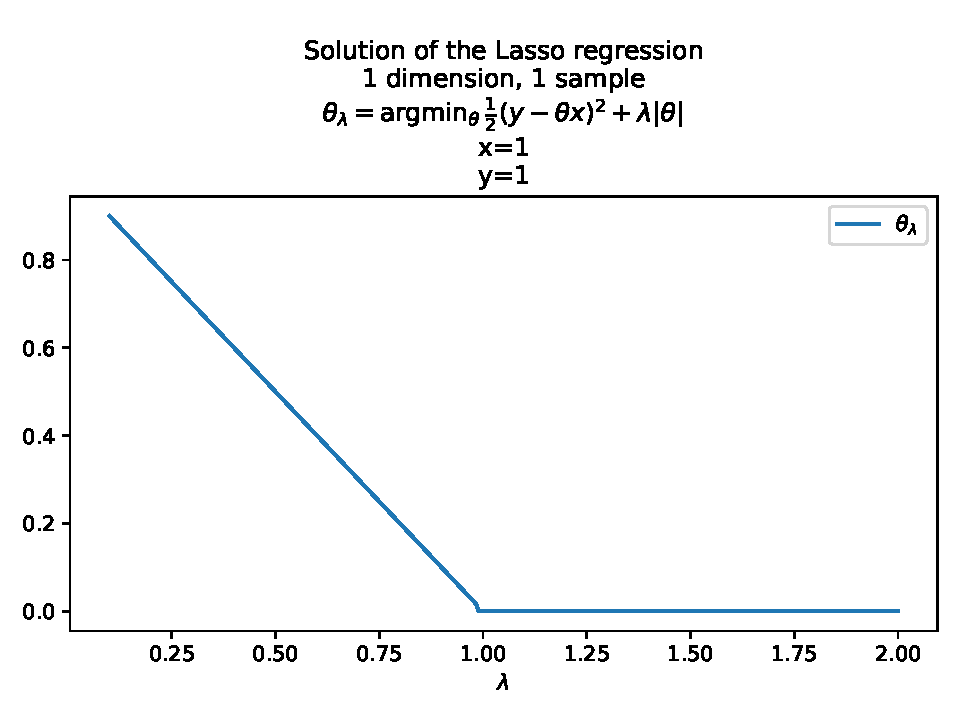
\includegraphics[width=1\textwidth]{lasso_regression_x_1_y_1}
    \caption{Solution of the one-dimensional Lasso estimator}
    \label{fig:lasso_regression_x_1_y_1}
\end{figure}

\tableofcontents

\pagebreak

\section{\large\color{Blue}General Lasso estimator}

Lasso regression is a regularization method for linear regression based on  the
L1 norm. With our usual notations, the Lasso estimator is the solution to the
following optimization problem:

\begin{equation}
    \tilde{\theta}_{\lambda}\in \argmin_{\theta\in \mathbb{R}^d}\{\frac{1}{2}||y-X\theta||^2+\lambda ||\theta||_1\}
\end{equation}

where

\begin{itemize}
    \item  $X\in \mathbb{R}^{n, d}$ is the design matrix.
    \item $y\in \mathbb{R}^{n}$ is the vector of labels
    \item  $\lambda\in \mathbb{R}_{+}$ is the regularization constant (called alpha in scikit-learn)
\end{itemize}

\section{\large\color{Blue}1D Lasso}

In this session we analyze the Lasso regression on a simple, one-dimensional
example, in order to develop the intuition of why this method leads to
\textbf{sparse} estimators. We hence consider the simplified problem:
    
    \begin{equation}
	\theta_{\lambda} = \argmin_{\theta}F_{\lambda}(\theta)
    \end{equation}

    with

    \begin{equation}
	F_{\lambda}(\theta) = \frac{1}{2}(y-\theta)^2+\lambda |\theta|
    \end{equation}

    and $y\in \mathbb{R}_{+}$, $\lambda\in \mathbb{R}_{+}$, $\theta\in \mathbb{R}$, where we assume that the input $x$ is equal to $1$ in order to lighten the notations.
    \\


    {\color{Purple}{Find the solution to the one-dimensional Lasso problem, as a function of $\lambda$. An example solution for $y=1$ is shown in figure \ref{fig:lasso_regression_x_1_y_1}.}

    \textbf{Remark:} in order to conclude on the optimal $\theta$ value as a function of $\lambda$, you can set an arbitrary value of $y$.

    Run a simulation that reproduces the plot shown in figure \ref{fig:lasso_regression_x_1_y_1} using scikit-learn.
}
\end{document}
